\chapter{Theoretical Foundations}
\label{chapter_Theoretical_Foundations}

% Introduction ST Domain and Data
In this work, we are interested in processes from Spatio--Temporal domains with high volumes of data. A feature of spatio--temporal data that distinguishes it from other data is the presence of dependencies among measurements induced by the spatial and temporal dimensions. The data instances are structurally related to each other in the context of space and time, showing varying properties in different spatial regions and time periods \cite{Atluri2018}. 

% ST Data Properties
Thus, space and time introduce a variety of spatio--temporal data types and representations. They have two generic properties: (i) auto-correlation, meaning that observations made at nearby locations and time stamps are not independent but are correlated with each other, and (ii) heterogeneity (or non-stationarity), both in space and time in varying ways and levels. These properties imply that spatial observations have consistent values at nearby locations, and show a smooth variation in temporal observations; as for the heterogeneity in space and time, it requires the learning of different models for varying spatio-temporal regions \cite{Wikle2019}.

% Introduction and Focus to Time Series -- Univariate
We are interested in spatio--temporal data with a representation that involves treating spatial locations as objects, as well as using the measurements collected from a spatial location over time to define the features. This type of data are called time-series; in particular we are interested in univariate time-series:

% Time Series definition
\begin{definition}[Time Series]
	An ordered sequence of values of a variable at equally spaced time intervals.
\end{definition}

\begin{definition}[Univariate time-series]
	A univariate time series is the simplest form of temporal data and is a sequence of real numbers collected regularly over time, where each number represents a value. Denoted by:
	\begin{equation}
	    \mathcal{S} = \left(s_{t}: \, t \in T \right)
	\end{equation}
	where $s_{t} \in \mathbb{R}$ and $T$ is the index set.
\end{definition}

Several applications represented by this type of data exist, and depending of the solution proposed for the problem studied, it is necessary to use specific techniques and methods. We focus in those used to identify groups of time series that show similar temporal activity and are located nearby in space. At the same time, we are interested in techniques that use time series as input features to predict a target variable, in order to generate models that can predict the value of a time series at a future time stamp using its historical values.

% Chapter Outline
In Sections \ref{Sec:TimeSeriesClustering} and \ref{Sec:TimeSeriesClassification}, we introduce methods and techniques designed to find groups of time-series with high similarity. 
%TODO \ref{Sec:TimeSeriesForecast}

\section{Clustering}
\label{Sec:TimeSeriesClustering}

% Clustering definition and applications
Clustering is a data mining technique where similar data are placed into related or homogeneous groups without advanced knowledge of the groups' definitions (unsupervised learning) \cite{HastieTF2009}. Given a similarity measure, clusters are formed by grouping objects that have maximum similarity with other objects within the group, and minimum similarity with objects in other groups. It is a useful approach for exploratory data analysis as it identifies structures in an unlabeled dataset by objectively organizing data into similar groups.

In the context of this work, according to \cite{Aghabozorgi2015}, time series clustering can be defined as follows:

\begin{definition} Time-series clustering: given a dataset of $n$ time-series data $\mathcal{D} = \{\mathcal{S}_1, \mathcal{S}_2, \ldots, \mathcal{S}_n\}$; the process of unsupervised partitioning of $\mathcal{D}$ into $\mathcal{C} = \{C_1, C_2, \ldots C_k\}$, in such a way
that homogenous time-series are grouped together based on a certain similarity measure, is called time-series clustering. Then, $C_i$ is called a cluster, where $\mathcal{D} = \bigcup_{i=1}^{k} C_{i}$ and $C_i \cap C_j \neq \emptyset$ for $i \neq j$.
\end{definition}

% Similarity Measure
%http://practicalquant.blogspot.com/2012/10/mining-time-series-with-trillions-of.html
We need to consider a similarity measure to calculate the similarity among the whole time-series. This is not a simple process, time-series data are naturally noisy and include outliers and shifts, in some cases the length of time-series varies and the distance among them needs to be calculated \cite{Pal2017}. In the literature, we found several approaches to find similarity among time-series. In this context, we chose shape--based approaches, where shapes of two time-series are matched as well as possible by a non-linear stretching and contracting of the time axes (considering raw time-series data).

\subsection{Shape-based Distance Algorithms}
\label{sec:ShapeBasedDistance}

Shape-based distance algorithms are usually employed in conventional clustering methods \cite{Pal2017}. These algorithms are compatible with static data while their distance/similarity measure has been modified with an appropriate one for time-series. A commonly used approach for calculating shape--based similarity measures is the Dynamic Time Warping (DTW) \cite{Sakoe1978} and its variants. DTW is a generalization of classical algorithms for comparing discrete sequences to sequences of continuous values, and leverages dynamic programming to calculate an optimal match between two sequences of feature vectors by allowing for stretching and compression of sections of the sequences. 

Given two time series, $\mathcal{S}_{1} =\left(s^{1}_{1}, s^{1}_{2}, \ldots, s^{1}_{n}\right)$ and $\mathcal{S}_{2} = \left(s^{2}_{1}, s^{2}_{2}, \ldots, s^{2}_{m}\right)$, DTW aligns the two series so that their difference is minimized. To this end, an $n \times m$ matrix, known as local cost matrix is computed, where the $(i, j)$ element of the matrix contains the distance $d(s^{1}_{i}, s^{2}_{j})$ between two points $s^{1}_{i}$, and $s^{2}_{j}$. Normally, the Euclidean distance is used here.

Once the local cost matrix is built, the algorithm finds an alignment path which runs through the low-cost area. This warping path defines the correspondence of an element $s^{1}_{i} \in \mathcal{S}_{1}$ to $s^{2}_{j} \in \mathcal{S}_{2}$, following the boundary condition which assigns the first and last elements of $\mathcal{S}_{1}$ and $\mathcal{S}_{2}$ to each other (See Figure \ref{Fig:DTW_warp_path}). Formally, the alignment path or warping path is the sequence $w = w_{1} , w_{2}, \ldots w_{k}, \ldots, w_{K}$ with $\max(m, n) \leq K \leq m + n-1$, where each $w$ is an element that satisfies three constraints: boundary condition, continuity, and monotonicity. 

\begin{figure}[htb]
	%\begin{minipage}[b]{0.8\textwidth}
	\centering
	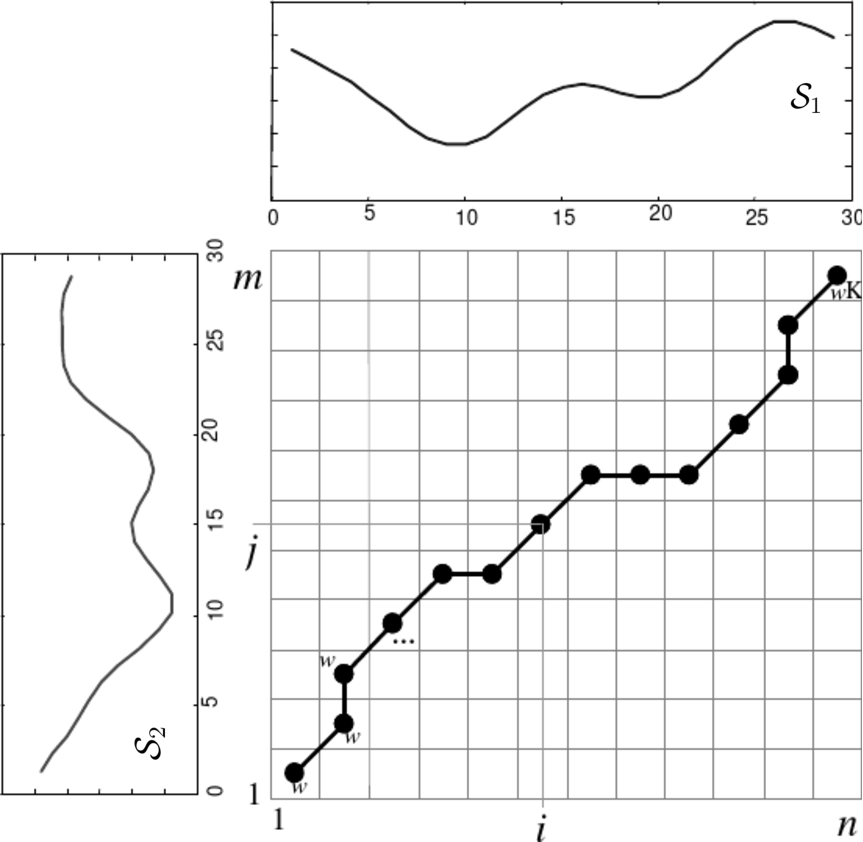
\includegraphics[scale=0.5]{../Figures/DTW-WarpPath}
	\caption{Time Series Warp Path.}
	\label{Fig:DTW_warp_path}
	%\end{minipage}
\end{figure}

The boundary condition constraint requires the warping path to start and finish in diagonally-opposite corner cells of the matrix. That is $w_{1} = (1, 1)$ and $w_{K} = (m, n)$. The continuity constraint restricts the allowable steps to adjacent cells. The monotonicity constraint forces the points in the warping path to be monotonically spaced in time. 

The cost function associated with a warping path computed with respect to the local cost matrix (which represents all pairwise distances) is defined by: 
\begin{equation}
    d_{w}\left(\mathcal{S}_{1}, \mathcal{S}_{2}\right) = \sum_{1}^{L} d(s^{1}_{nl}, s^{2}_{ml}).
\end{equation}

The warping path which has a minimal cost associated with alignment called the optimal warping path.  This will be called path $w^{*}$. By following the optimal warping path definition in order to find one, we need to test every possible warping path between $\mathcal{S}_{1}$ and $\mathcal{S}_{2}$. This could be computationally challenging due to the exponential growth of the number of optimal paths as the lengths of $\mathcal{S}_{1}$ and $\mathcal{S}_{2}$ grow linearly. To overcome this challenge, DTW employs an algorithm based on Dynamic Programming, with computational complexity of only $\bigO(mn)$.

The Dynamic Programming part of DTW algorithm uses the DTW distance function:
\begin{equation}
DTW(\mathcal{S}_{1}, \mathcal{S}_{2}) =d_{w^{*}}(\mathcal{S}_{1}, \mathcal{S}_{2}) = \min\left\{d_{w}(\mathcal{S}_{1}, \mathcal{S}_{2}), w \in W^{n\times m} \right\}
\end{equation}

where $\mathcal{S}_{1}$ and $\mathcal{S}_{2}$ are the input time series and $W^{n\times m}$ is the set of all possible warping paths. We define $D$ as the accumulated cost matrix representing all the pairwise distances between $\mathcal{S}_{1}$ and $\mathcal{S}_{2}$; the algorithm then builds $D$ as follows:
\begin{enumerate}
    \item First row: $D(1, j) =\sum_{k=1}^{j}d(s^{1}_{1}, s^{2}_{k}), j \in [1, m]$.
    \item First column: $D(i,1) =\sum_{k=1}^{i}d(s^{1}_{k}, s^{2}_{1}), i \in [1, n]$.
    \item All other elements: $D(i, j) = \min \left\{ D(i-1, j-1), D(i-1, j), D(i, j-1)\right\} + d(s^{1}_{i}, s^{2}_{j}), i \in [1, n], j \in [1, m])$.
\end{enumerate}

The time cost of building this matrix is $\bigO(mn)$, and this same computational complexity represents the DTW algorithm as a whole. Once the accumulated cost matrix $D$ is built, the warping path can be found by the simple backtracking from the point $w_{end} = (m,n)$ to the $w_{start} = (1,1)$ following the greedy strategy as described by the Algorithm \ref{Alg:OptimalWarpingPath} \cite{Senin2008}.

\begin{algorithm}
\caption{Optimal Warping Path (dtw)} 
\label{Alg:OptimalWarpingPath}
\begin{algorithmic}[1]

\State $path[] \gets newarray$;
\State $i:=rows(dtw)$;
\State $j:=columns(dtw)$;
\While {$(i >1) \,\, \&\,\, (j >1)$}
    \If {$i ==  1$} 
        \State $j \gets j-1$
    \ElsIf {$j == 1$}
        \State $i \gets i-1$
    \Else 
        \If{$dtw(i-1, j) == \min \{dtw(i-1, j); dtw(i, j-1); dtw(i-1, j-1)\}$}
            \State $i \gets i-1$
            \ElsIf {$dtw(i, j-1)  ==  \min\{dtw(i-1, j); dtw(i, j-1); dtw(i-1, j-1)\}$}
                \State $j \gets j-1$
            \Else
                \State $i \gets i-1$
                \State $j \gets j-1$
        \EndIf
    \State $path.add((i, j))$
    \EndIf
\EndWhile
\State \textbf{return} $path$  
\end{algorithmic}
\end{algorithm}

%TODO Finishing paragraph

\subsection{$k$--Medoids Clustering }
\label{Sec:kMedoidsClustering}

% K-means
A cluster analysis method makes $k$ groups from $n$ unlabeled objects in the way that each group contains at least one object. One of the most used algorithms of clustering is $k$-Means, where each cluster has a representative which is the mean value of its objects. The main idea behind $k$-Means clustering is the minimization of the total distance (typically Euclidean distance) between all objects in a cluster from their cluster center (representative).

Another member of partitioning family is $k$--Medoids method, with its corresponding default implementation Partition Around Medoids (PAM), where the representative of each cluster is one of the nearest objects to the center of the cluster \cite{Kaufman2009}. $k$-Means and $k$-Medoids algorithms make clusters which are constructed in a `crisp' manner, meaning that an object is either a member of a cluster or it is not.

In the case of time-series clustering, the prototype or representative of each cluster is called optimal Steiner sequence, and it is defined as a sequence which minimizes the sum of squared distances to other objects within the cluster \cite{Kaufman2009}. Given time-series in a cluster, the distance of all time-series pairs within the cluster is calculated using a distance measure, such as Euclidean or DTW distance. Then, one of the time-series in the cluster, which has lower sum of square error is defined as medoid of the cluster.

In this work, instead of the default PAM implementation of k-medoids, we use an alternative algorithm that requires a distance matrix of all the pairwise distances between points \cite{Park2009}. The procedure can be described as follows:

\begin{enumerate}
    \item \textbf{Preparation:} the distance matrix is calculated once and made available to the following steps.
    \item \textbf{Initialization:} randomly select $k$ of the $m$ data points as the medoids.
    \item \textbf{Assignment:} associate each data point to the closest medoid, based on the distance measure. This can be achieved by finding the minimum value at the corresponding row of the distance matrix.
    \item \textbf{Update:} for each medoid $j$ and each data point $i$ associated with $j$, swap $j$ and $i$ and compute the total cost of the configuration (which is, the average dissimilarity of $i$ to all the data points associated to $j$). 
    Select the medoid $j$ with the lowest cost of the configuration. Iterate between steps 3 and 4 until there is no change in the assignments.
\end{enumerate}


% Considering varying k partitions
The $k$--Medoids approach is a seed based algorithm, this means that the performance is dependent on initial cluster center selection and the optimal number of clusters \cite{Chowdhury2019}. The convergence of this algorithm primarily depends on the initialization phase, when the membership of each data point is calculated. The algorithm not only produces different clustering results for different values of $k$, but also for different values of the initial seed. In addition, increasing $k$ will always reduce the $k$--Medoids cost (within-cluster sum of squares, or WSS) in the resulting grouping, to the extreme case of zero cost if each data point is considered its own cluster (i.e., when $k$ equals the number of data points) \cite{HastieTF2009}. 

In $k$--Medoids clustering algorithm, the number of clusters $k$, has to be pre-assigned, which may not be readily available or may not be easily easily determined for many applications. Thus, one of the main drawbacks of $k$--Medoids is the difficulty in obtaining natural clustering results when working with static objects \cite{Mohri2012}.

The issue of requiring a pre-assigned value for the number of clusters $k$ is exacerbated when applying the $k$--Medoids method on time-series data, because the datasets are very large and diagnostic checks for determining the number of clusters is not easy \cite{Aghabozorgi2015}. In Section \ref{Sec:Selectk}, we will explore methods and techniques to find the optimal number of $k$ under these conditions.

\section{Time Series Classification} 
\label{Sec:TimeSeriesClassification}

Classification is a type of Supervised Learning, where the learning dataset instances are tuples (attributes, label), ``attributes'' represent the input data and ``label'' represents the target output. The goal of the classification process is to build a system that, given a new input, is able to predict a target output \cite{Mohri2012}. 

For Time Series Classification, we consider the data points as the whole time series, and the task consists of predicting its correct label. In \cite{Fawaz2019}, the problem of time-series classification is defined as follows: 

\begin{definition}
A dataset $D=\{(\mathcal{S}_1,Y_1),(\mathcal{S}_2,Y_2), \ldots ,(\mathcal{S}_N,Y_N)\}$ is a collection of pairs $(\mathcal{S}_i,Y_i)$ where $\mathcal{S}_i$ is univariate time series with $Y_i$ as its corresponding one-hot label vector.  For a dataset containing $k$ classes, the one-hot label vector $Y_i$ is a vector of length $k$ where each element $j \in [1,k]$ is equal to 1 if the class of $X_i$ is $j$ and $0$ otherwise.
\end{definition}

Traditional classification approaches can provide a basic baseline for solving this underlying time-series classification task. However the past two decades, research has shown that designing algorithms that can exploit the temporal information are very useful to achieve high classification accuracy \cite{Wang2017}. In particular, the use of Deep Learning methods to solve time-series classification problems are gaining more adepts, due to capacity to work with sequential data \cite{Bagnall2017a, Zhao2017, Zebik2017}.

\subsection{Deep Learning for Time Series Classification}
\label{Sec:DL-TSC}
% Intro to deep learning for time series classification
In this work, we consider the use of Neural Network Classifiers. Traditional machine learning systems require considerable domain expertise and careful hand engineering to come up with a feature extractor that transforms the raw data (such as pixel values of an image) into a suitable internal representation, or feature vector, from which a learning system (such as a classifier) can detect or classify patterns in the input \cite{Guyon2006}. 

A Deep Learning approach, allows inputting the raw data to the learning algorithm without first extracting features or defining a feature vector. Instead of handcrafting a set of rules and algorithms to extract features from raw data, deep learning involves learning these features automatically during the training process \cite{Goodfellow2016, Schmidhuber2015}. 

A deep learning network is designed to learn hierarchical representations of the data. Learning takes place via submodels structured in the form of layers stacked on top of each other. Given that deep learning networks have typically more layers and parameters than other neural networks, they have the potential to represent more complex inputs. Figure \ref{Fig:TSC-Fawaz} represents a general deep learning framework for Time-Series Classification, where the input is shown as a set of $M$ univariate time series, and the output as a probability distribution over $K$ classes into which the series are classified.

\begin{figure}[htb]
	%\begin{minipage}[b]{0.8\textwidth}
 	\centering
 	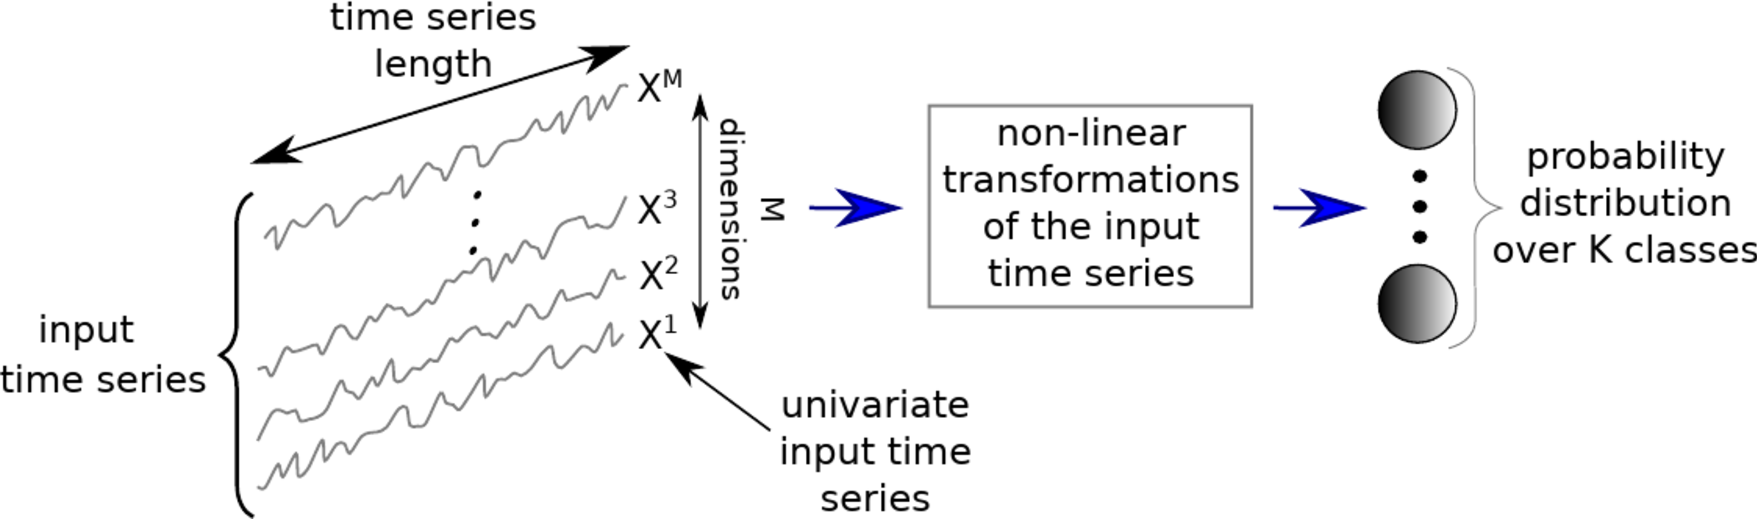
\includegraphics[scale=0.5]{../Figures/TSC_Fawaz}
 	\caption{Deep Learning Framework for Time-Series Classification \cite{Fawaz2019}.}
 	\label{Fig:TSC-Fawaz}
 	%\end{minipage}
\end{figure}

In \cite{Fawaz2019}, the composition of a deep neural network (DNN) is described as follows: there are $L$ parametric functions referred to as layers, where each layer is considered a representation of the input domain. A layer $l_{i}$, where $i \in 1, \ldots L$, contains neurons which are units of computation that calculate one element of the layer's output. Each layer $l_i$ takes as input the output of its previous layer $l_{i-1}$, and applies a nonlinearity (such as the sigmoid function) to compute its own output.

The behavior of these non-linear transformations is controlled by a set of parameters $\theta_{i}$ for each layer. In the context of a DNN, these parameters are called weights, which link the input of the previous layer to the output of the current layer. Hence, given an input $x$, a neural network performs the following computations to predict the class:
\begin{equation}
f_{L}(\theta_{L}, x) = f_{L-1}(\theta_{L-1}, f_{L-2}(\theta_{L-2}, \ldots, f_{1}(\theta_{1},x)))
\end{equation}
where $f_{i}$ corresponds to the non-linearity applied at layer $l_{i}$. This process is known as the feed-forward propagation in the deep learning literature \cite{Goodfellow2016}.

% Architectures for time-series classification
We consider two Neural Network architectures for sequential data: the Long-Short Term Memory Neural Network (LSTM) \cite{HochSchm1997} which is a type of Recurrent Neural Network (RNN) \cite{Rumelhart1986a}, and the Convolutional Neural Network (CNN) \cite{Lecun1989}.

% RNN
The family of Recurrent neural networks (RNNs) are a class of artificial neural network architecture. They are inspired by the cyclical connectivity of neurons in the brain and use iterative function loops to store information. RNNs have several properties that make them an attractive choice for sequence labeling; in particular, they are flexible in their use of context information because they can learn what to store and what to ignore.

% LSTM 
One major drawback of RNNs is that the range of contextual information is limited and the Back-Propagation through time does not work properly. This is noticeable in either vanishing or exploding outputs of the network. In the literature, this problem is called vanishing gradient problem or exploding gradient \cite{Glorot2011}. When the network is learning to bridge long time lags, it may take a large amount of time or not even work at all, because of the vanishing gradient problem. The exploding gradient leads to oscillating weights, which also reduces the quality of the network. 

To address these problems, Hochreiter and Schmidhuber introduce a gradient-based method called ``Long Short-Term Memory Neural Networks'' or LSTM \cite{HochSchm1997}. By extending the memory, LSTM enables RNNs to remember inputs over a long period of time, thereby creating relationships with long-term dependencies. This is because LSTMs contain information in a `memory', which gives the ability of read, write and delete information from it.

A unit memory in LSTM can be seen as a gated cell, shown in Figure \ref{Fig:LSTM-Unit}. The three gates determine whether or not to let new input in (input gate), delete the non important information (forget gate), or let it impact the output at the current time-step (output gate). The decision to open a gate (and thus perform one of the three actions) is based on the importance that the cell assigns to the information. The assignment of importance is realized through weights, which are also learned by the algorithm. As a result, a cell can learn over time which piece of information is important and which is not. The gates in an LSTM are analog in the form of sigmoids, meaning they range from zero to one. The fact that they are analog enables them to do back-propagation.

\begin{figure}[htb]
	%\begin{minipage}[b]{0.8\textwidth}
	\centering
	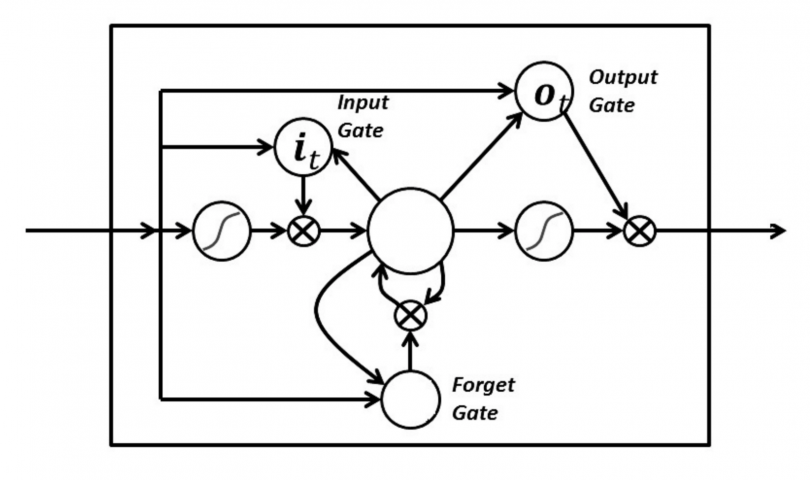
\includegraphics[scale=0.4]{../Figures/rnn-three-gates}
	\caption{A unit in a LSTM architecture with three gates: input, forget and output gate. }
	\label{Fig:LSTM-Unit}
	%\end{minipage}
\end{figure}

% CNN
Convolutional Neural Networks (CNNs) \cite{Lecun1989} are a subset of machine learning techniques that uses multi-layered artificial neural networks to deliver state-of-the-art accuracy in tasks such as object detection, speech recognition, language translation and others \cite{Szegedy2013}. CNNs employ filters within convolutional layers to transform data, whereas RNNs reuse activation functions from other data points in the sequence to generate the next output in a series. 

The process of a convolution layer can be better explained in the context of image processing: a convolution operation is performed as a window of weights sliding across an image, where an output pixel produced at each position is the weighted sum of the input pixels covered by the window. The weights that parameterize the window remain the same throughout the scanning process. Therefore, convolutional layers can capture the shift-invariance of visual patterns and learn robust features.

\begin{figure}[htb]
	%\begin{minipage}[b]{0.8\textwidth}
	\centering
	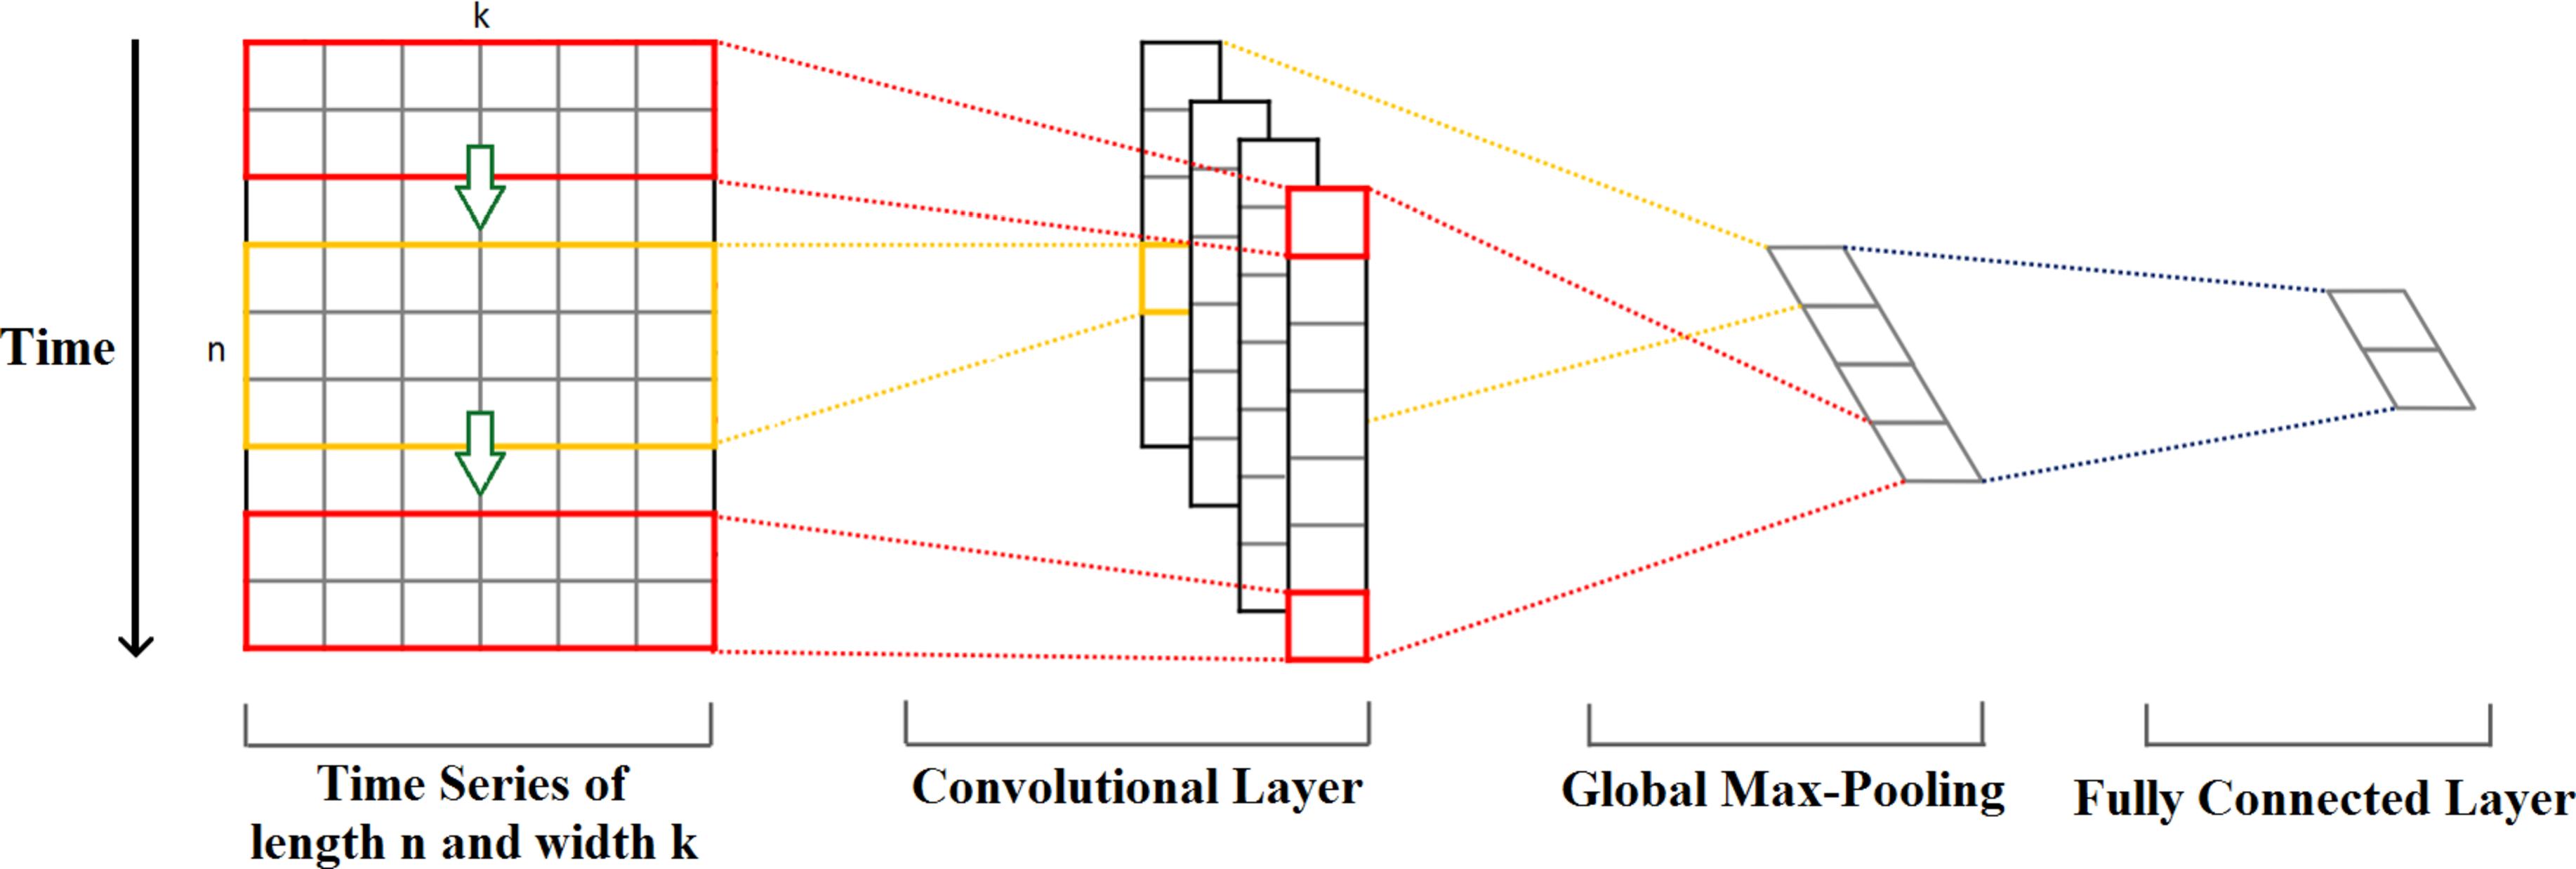
\includegraphics[scale=0.25]{../Figures/1d-cnn}
	\caption{1D Convolution Network for Time Series \cite{Kim2014}.}
	\label{Fig:1DCNN}
	%\end{minipage}
\end{figure}

Multilayer Feed Forward or fully connected layer is a structure where neurons from a layer are connected to all the neurons in the next layer, for a multiclass classification the dense layer is commonly used. Considering the \texttt{softmax} function onto the last layer, it creates a probability distribution over $K$ classes, and produces an output vector of length $K$. Each element of the vector is the probability that the input belongs to the corresponding class. The most likely class is chosen by selecting the index of that vector having the highest probability (See Figure \ref{Fig:1DCNN}).

% Hybrid models LSTM-CNN
The main difference between CNN and RNN is the ability to process temporal information or data that comes in sequences, such as a sentence for example. Moreover, convolutional neural networks and recurrent neural networks are used for completely different purposes, and there are differences in the structures of the neural networks themselves to fit those different use cases. 

While RNNs and CNNs have several differences, they are not completely mutually exclusive. It is possible use them together for increased effectiveness. This can especially be helpful when the input has to be classified as visually complex with temporal characteristics. In this context, a CNN can be used to handle spatial data, while RNN can be leveraged to process the temporal aspect of the data. In a combined network, the input is first passed through the CNN layers and then its output is fed to the RNN network layer. These hybrid structures are being currently used for applications like gesture recognition, video scene labeling, video identification, and DNA sequencing. In this work, we will analyze the applicability of a CNN, a RNN and the hybrid approach for time series classification.

\section{Time Series Analysis and Forecast}
\label{Sec:TimeSeriesForecast}

% Spatio-Temporal Modeling
The basic objective of predictive learning methods is to learn a mapping from the input features (also called independent variables) to the output variables (also called dependent variables) using a representative training set. In spatio-temporal (ST) applications, both the input and output variables can belong to different types of ST data instances, thus resulting in a variety of predictive learning problem formulations.

% TS and UTS Data Recap to Introduce TSA
A successful utilization of time series data would lead to monitoring the evolution of a phenomenon over time. The field of time series analysis aims to utilize such data for several purposes that can be categorized as: to understand and interpret the underlying forces that produce the observed state of a system or process over time; to forecast the future state of the system or process in terms of observable characteristics.

% TS Data Characteristics for modeling
The nature of time-series data includes the following properties: i) large in data size, ii) high dimensionality and iii) continuously updated. Moreover, time-series data, being characterized by its numerical and continuous nature, should not be manipulated using each individual numerical value as it was independent from the series \cite{Pal2017}. Instead, we want to explore the following three characteristics of time-series:

\begin{itemize}
	\item Trend: A trend exists when there is a long-term increase or decrease in the data. It does not have to be linear. Sometimes we will refer to a trend as ``changing direction'', when it might go from an increasing trend to a decreasing trend.
	\item Seasonal: A seasonal pattern occurs when a time series is a effected by seasonal factors such as the time of the year or the day of the week. Seasonality is always of a fixed and known frequency. 
	\item Cyclic: A cycle occurs when the data exhibit rises and falls that are not of a frequency.
\end{itemize}

\subsection{Methods for Time Series Analysis}
\label{Sec:MethodsTSA}

% Introduction TSA
A foundational objective of time series analysis is to develop models that provide plausible descriptions for time series data. For this we consider the fact that time series data are usually not independent and the analysis must take into account the time order of the observations. As a consequence, when successive observations (time series) are dependent, future values may be predicted from past observations \cite{Mills2019}. 
% FIXME "stochastic" needs rigorous definition
% TODO https://stats.stackexchange.com/questions/126791/is-a-time-series-the-same-as-a-stochastic-process
Many applications are represented by stochastic time series, meaning that the future is partly determined by past values. Thus the exact predictions are impossible to determine and must be replaced by the idea that future values have a probability distribution, which is conditioned on a knowledge of past values. 

There are several possible objectives in analyzing a time series, in particular time-series forecasting is a form of quantitative forecasting. It can be applied when three conditions exist: (1) Information about the past is available, (2) this information can be quantified in the form of numerical data, and (3) it can be assumed that some aspects of the past pattern will continue into the future. This last condition is known as the ``assumption of continuity'' \cite{Makridakis2008}; it is an underlying premise of all quantitative forecasting methods. 

Time series forecasting treats the system as a black box and makes no attempt to discover the factors affecting its behavior. Therefore, prediction of the future is based on past values of a variable and/or past errors, but not on explanatory variables which may affect the system. The objective of such time series forecasting methods is to discover the pattern in the historical data series and extrapolate that pattern into the future. 
In this work we consider Auto Regressive Integrated Moving Average (ARIMA) as the main time--series forecast method to generate predictive models.

\subsubsection{Auto Regressive Integrated Moving Average}
\label{Sec:TheoryARIMA}

% ARIMA for time series forecast
ARIMA are the most general class of models for forecasting a time series which can be made to be ``stationary'' by differencing (when necessary). A random variable (in this case, a time series), is said to be stationary if its statistical properties (mean and covariance) are constant over time.  A stationary series has no trend, its variations around its mean have a constant amplitude, and its autocorrelations (correlations with its own prior deviations from the mean) remain constant over time.  A random variable of this form can be usually viewed as a combination of signal and noise, and the signal (if one is apparent) could be a pattern of fast or slow mean reversion, or sinusoidal oscillation, %or rapid alternation in sign,
and it could also have a seasonal component. An ARIMA model can be viewed as a ``filter'' that tries to separate the signal from the noise; this signal can then be extrapolated into the future to obtain forecasts \cite{Chatfield2019}.

In a multiple regression model, the variable of interest is predicted using a linear combination of predictors. In an autoregression model, the forecast of the variable of interest is performed using a linear combination of past values of the variable. The term autoregression indicates that it is a regression of the variable against itself. Autoregressive models are based on the idea that the current value of the series, $s_{t}$, can be explained as a function of $t_{p}$ past values, $s_{t-1}, s_{t-2}, \ldots, s_{t-p}$, where $t_{p}$ determines the number of steps into the past needed to forecast the current value. 

Thus, an autoregressive (AR) model of order $p$ can be written as 
\begin{equation}
    \label{Eq:AR_p}
    s_{t} = c + \phi_{1} s_{t-1} + \phi_{2} s_{t-2} + \ldots +\phi_{p}s_{t-p} + \varepsilon_{t},
\end{equation} where $\varepsilon_{t}$ is white noise. This is like a multiple regression but with lagged values of $s_{t}$ as predictors. We refer to this as an AR$(p)$ model, an autoregressive model of order $p$. Autoregressive models are remarkably flexible at handling a wide range of different time series patterns. Changing the parameters $\phi_{1},\ldots, \phi_{p}$ results in different time series patterns. The variance of the error term $\varepsilon_{t}$ will only change the scale of the series, not the patterns.

Rather than using past values of the forecast variable in a regression, a moving average (MA) model uses past forecast errors in a regression-like model. 
\begin{equation}
    \label{Eq:MA_q}
    s_{t} = c + \varepsilon_{t} + \theta_{1} \varepsilon_{t-1} + \theta_{2}\varepsilon_{t-2} + \ldots + \theta_{q} \varepsilon_{t-q},    
\end{equation}
 where $\varepsilon_{t}$ is white noise. We refer to this as an MA$(q)$ model, a moving average model of order $q$. Notice that each value of $s_{t}$ can be thought of as a weighted moving average of the past few forecast errors.

Combining differencing with autoregression and a moving average model, a non-seasonal ARIMA model is obtained. This model can be written as:
\begin{equation}
    \label{Eq:ARIMApdq}
    s^{'}_{t} = c + \phi_{1} s^{'}_{t-1} + \ldots + \phi_{p} s^{'}_{t-p} + \theta_{1}\varepsilon_{t-1} + \ldots + \theta_{q} \varepsilon_{t-q} + \varepsilon_{t},
\end{equation}
where $s^{'}_{t}$ is the differenced series (it may have been differenced more than once). The ``predictors'' on the right hand side include both lagged values of $s_{t}$ and lagged errors. We call this an ARIMA$(p,d,q)$ model, where
\begin{itemize}
    \item $p =$ order of the autoregressive part;
    \item $d =$ degree of first differencing involved;
    \item $q =$ order of the moving average part. 
\end{itemize}

% TODO revisar integrated vs differencing components
% The integrated components are useful when data has non-stationarity, and the integrated part of ARIMA helps in reducing the non-stationarity. 
In summary, the ARIMA forecasting equation for a stationary time series is a linear (i.e., regression-type) equation in which the predictors consist of lags of the dependent variable and/or lags of the forecast errors.  The integrated components are useful when data has non-stationarity, and the integrated part of ARIMA helps in reducing the non-stationarity. The ARIMA applies differencing on time series one or more times to remove non-stationarity effect. The $(p, d, q)$ tuple represents the order for AR, the differencing component, and the order for MA, respectively. Viewed in another way, the $d$ component aims to detrend the signal to make it stationary and ARMA model can be applied to the de--trended dataset \cite{Hyndman2018}.

When working with ARIMA models, the $(p, d, q)$ tuple has to be specified, and different combinations of values will produce results with varying accuracy. An approach to tackle the problem of choosing adequate parameters is to use the auto ARIMA procedure. It performs a grid search that selects the $(p, d, q)$ model parameters based on the minimization of the AIC (Akaike Information Criterion), given by the following formula \cite{Hyndman2008}:

\begin{equation}
\mathrm{AIC} \, = \, 2(p + q+ k + 1) - 2\ln(\hat L)
\end{equation}

where $k$ is the number of estimated parameters and $\hat{L}$ is the maximum value of the likelihood function for the model. In this way, the grid search will try to maximize the goodness of the fit, while penalizing complex models with high-valued parameters \cite{Hyndman2018}.

\subsubsection{$k$ Nearest Neighbor}
\label{Sec:TheorykNN}

Another method considered in this work for time series forecasting is the $k$ Nearest Neighbor (kNN) regression. $k$NN is a nonparametric classification method, based on the measurement of a point's similarity to a training set containing patterns for which class labels are supplied. $k$NN is a memory-based method and does not build a model through learning. Instead, the classification is made by aggregating the values provided by the training patterns in the vicinity of the current point \cite{Altman1992}. 

When $k$NN is applied to time series forecasting, it is necessary to:
\begin{itemize}
    \item choose the concrete similarity functions used to find the closest neighbors,
    \item decide how to effectively produce the prediction.
\end{itemize}
For the former step, let $\{s_{1}, s_{2}, \ldots, s_{n}\}$ be the series to be analyzed. We search for $k$ subsequences of length $t_p$ inside the given series, that are closest to the suffix vector $\{s_{n-t_{p}+1},\ldots, s_{t}\}$, with $t_{p} >1$. These $k$-subsequences are of the form: 
\begin{equation*}
    \{s_{q_{1}}, s_{q_{1}+1}, \ldots, s_{q_{1}+t_{p}-1} \}, \ldots \ldots, \{s_{q{k}}, s_{q_{k}+1}, \ldots, s_{q_{k} + t_{p} -1} \}
\end{equation*}

where $1 \leq q_{i} \leq n - t_{p}$, $i = \{1, 2, \ldots, k\}$. The values $k$ and $t_{p}$ are parameters of the prediction model \cite{Ban2013}. Here, it is possible to utilize the DTW similarity measure to compute the distances between series' suffix and a neighbor.

\subsection{Time Series Forecast Error}
\label{Sec:ErrorTSA}

% Time Series Forecast Error 
Accuracy measures, error statistics or measures, and loss functions are alternative ways of conveying information about the ability of a certain forecasting method to predict actual data, either when a model is fitted to such data, or for future periods (post-sample) whose values have not been used to develop the forecasting model \cite{Makridakis1993}. In order to represent the accuracy of forecast methods applied to univariate time series data, we use $s_{t}$ to denote the observation at time $t$, and $\hat{s}_t$ to denote the forecast of $s_{t}$.

In this work, we consider the following scale-dependent errors:
\begin{itemize}
	\item Mean Squared Error (MSE): Measures the average squared error of the predictions. For each point, it calculates the square difference between the predictions and the target, and then averages those values:
	\begin{equation}
	MSE = \frac{1}{n} \sum_{t=1}^{n} \left(s_t - \hat{s}_t\right)^{2}.
	\end{equation}
	
	The higher this value, the worse the prediction is considered to be. It is never negative, since we're squaring the individual prediction-wise errors before summing them, but would be zero for a perfect model.
	
	\item Root Mean Squared Error (RMSE): Represents the sample standard deviation of the differences between predicted and observed values (called residuals). It is calculated using the following formula:
	\begin{equation}
	RMSE = \sqrt{\frac{1}{n} \sum_{t=1}^{n} \left(s_t - \hat{s}_t\right)^2}
	\end{equation}
	Often, the RMSE is preferred to the MSE as it is on the same scale as the data. Historically, the RMSE and MSE have been popular largely because of their theoretical relevance in statistical modeling. However, they are more sensitive to outliers.
\end{itemize}

Additionally, we consider percentage errors, which have the advantage of being unit-free, and thus are frequently used to compare forecast performances between data sets. Measures based on percentage errors have the disadvantage of being infinite or undefined if $s_{t}=0$ for any $t$ in the period of interest, and having extreme values if any $s_{t}$ is close to zero. In this context, we consider the Mean Absolute Percentage Error (MAPE). Another problem with percentage errors that is often overlooked is that they assume the unit of measurement has a meaningful zero \cite{Hyndman2006}. This observation led to the use of the so-called ``symmetric'' MAPE (sMAPE) \cite{Makridakis1993}:

\begin{itemize}	
	\item Mean Absolute Percentage Error (MAPE):
	\begin{equation}
	MAPE = \frac{100}{n}\sum_{t=1}^{n} \frac{\left|s_t - \hat{s}_t\right|}{|s_t|}
	\end{equation}	
	\item Symmetric Mean Absolute Error (sMAPE):	
	\begin{equation}
	sMAPE = \frac{200}{n}\sum_{t=1}^{n} \frac{\left|s_t - \hat{s}_t\right|}{\left(s_{t}+\hat{s}_{t}\right)}
	\end{equation}	
\end{itemize}
In sMAPE The absolute difference between $s_{t}$ and $\hat{s}_{t}$ is divided by half the sum of absolute values of the actual value $s_{t}$ and the forecast value $\hat{s}_{t}$. The value of this calculation is summed for every fitted point $t$ and divided again by the number of fitted points $n$. In contrast to the MAPE, sMAPE has both a lower bound and an upper bound. The formula above provides a result between $0\%$ and $200\%$. However a percentage error between $0\%$ and $100\%$ is much easier to interpret.  

\section{Final Considerations}
\label{Sec:TheoFinalConsiderations}

% 
